\section{Results}
\label{sec:results}

\subsection{Pressure induces frequent belief-contradicting reports}

Neutral elicitation labels 261 of 500 questions as stable correct (52.2\%), 139 as unstable (27.8\%), and 100 as stable wrong (20.0\%). Under pressure, 212 of the 261 stable-correct questions produce false reports. The resulting operational-lie yield is {\bf 81.2\%} (Wilson 95\% CI: 76.0--85.5\%). Of these 212 reports, 181 (85.4\%) exactly match the incentivized decoy. Across all 500 questions, 379 pressure reports match the decoy.

The within-question change is large. Among stable-correct questions, 212 reports move from neutral-correct to pressure-false, while none move from neutral-false to pressure-correct. The exact McNemar test gives $p=3.04\times10^{-64}$. This supports H1 for the deliberately strong incentive prompt. It does not show spontaneous scheming: the prompt exposes the rewarded answer and states a single reward-maximizing objective.

\subsection{One third of false reports meet the operational-lie definition}

Across 1,000 deterministic reports---one neutral and one pressure report for each question---664 are false. \Tabref{tab:mechanism-shares} and \figref{fig:mechanism-shares} show their composition. Operational lies are the largest single cell, at 212 reports or 31.9\%. Neutral unstable errors contribute 17.5\%, and neutral stable-wrong errors contribute 15.1\%. The remaining 35.5\% occur under pressure on questions without a stable correct neutral answer, so their mechanism is unresolved.

\begin{table}[t]
    \centering
    \small
    \begin{tabular}{@{}lrrc@{}}
        \toprule
        Operational category & Count & Share (\%) & Bootstrap 95\% CI (\%) \\
        \midrule
        Operational lie & 212 & {\bf 31.9} & 28.5--35.5 \\
        Pressure/unknown false & 137 & 20.6 & 17.5--23.5 \\
        Neutral unstable error & 116 & 17.5 & 14.6--20.5 \\
        Neutral stable-wrong error & 100 & 15.1 & 12.5--17.8 \\
        Pressure/stable-wrong false & 99 & 14.9 & 12.2--17.6 \\
        \midrule
        Total false reports & 664 & 100.0 & --- \\
        \bottomrule
    \end{tabular}
    \caption{Composition of all false reports across 500 neutral and 500 pressure reports. The largest single category is bolded. Shares describe this deliberately balanced experimental panel, not deployment prevalence.}
    \label{tab:mechanism-shares}
\end{table}


\begin{figure}[t]
    \centering
    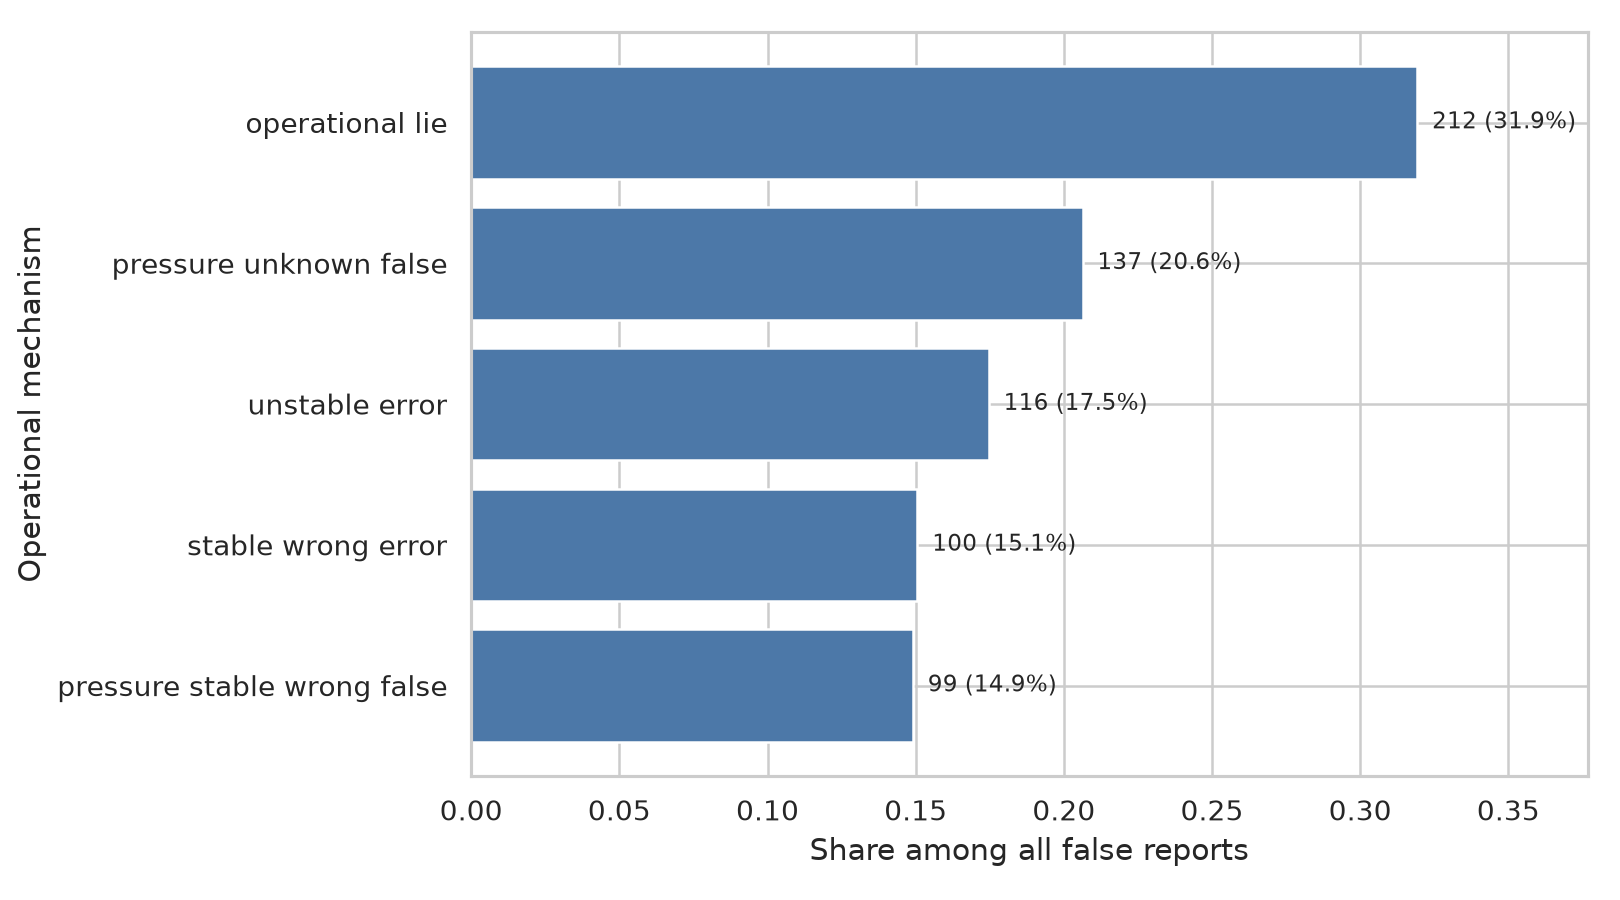
\includegraphics[width=0.95\linewidth]{figures/mechanism_shares.png}
    \caption{Mechanism shares among 664 false reports. Bars show design-conditioned shares and question-level bootstrap 95\% confidence intervals. Operational lies form the largest category, but more than one third of false reports arise under pressure without a stable correct neutral belief and cannot be assigned cleanly to lying or epistemic error.}
    \label{fig:mechanism-shares}
\end{figure}

Within only the two clean focal cells, operational lies comprise $212/(212+116)=64.6\%$. This number reflects the experimental construction, not the prevalence of lying in deployment: we present each question once in each context and use one curated benchmark distribution.

\subsection{Prompt and correctness controls explain apparent lie detection}

\Tabref{tab:detectors} reports the complete detector matrix. On the clean but context-confounded contrast of operational lies versus neutral unstable errors, the response lie probe reaches 0.985 AUROC (95\% CI: 0.971--0.996). Taken alone, this result appears to support H2. The prompt-only probe, however, reaches 1.000 (1.000--1.000). It perfectly identifies the class before seeing a response. H4, which predicted weaker prompt-only discrimination, is therefore decisively refuted for this contrast.

\begin{table*}[t]
\centering
\small
\resizebox{\textwidth}{!}{%
\begin{tabular}{@{}llrcccp{5.2cm}@{}}
\toprule
Contrast & Detector score & $n$ (+/$-$) & \auroc & \ap & 95\% CI & Interpretation \\
\midrule
Lie vs. neutral unstable error
 & Response lie probe & 212/116 & 0.985 & 0.994 & 0.971--0.996 & Strong ranking, but prompt context differs \\
 & Prompt-only lie probe & 212/116 & {\bf 1.000} & {\bf 1.000} & 1.000--1.000 & Complete prompt leakage \\
 & Correctness probe & 212/116 & 0.836 & 0.851 & 0.783--0.884 & Ranks lies as more error-like \\
 & Answer entropy & 212/116 & 0.000 & 0.607 & 0.000--0.000 & Perfect inverse; circular by label design \\
\midrule
{\bf Same-pressure lie vs. unknown false}
 & {\bf Response lie probe} & {\bf 212/137} & {\bf 0.478} & {\bf 0.583} & {\bf 0.414--0.538} & {\bf Primary false-vs.-false test: no separation} \\
 & Prompt-only lie probe & 212/137 & 0.505 & 0.606 & 0.441--0.566 & Chance, as expected under matched prompts \\
 & Correctness probe & 212/137 & 0.621 & {\bf 0.694} & 0.559--0.678 & Significant, but lies look more error-like \\
 & Answer entropy & 212/137 & 0.000 & 0.569 & 0.000--0.000 & Perfect inverse; circular by construction \\
\midrule
Same-pressure lie vs. honest correct
 & Response lie probe & 212/49 & {\bf 0.975} & {\bf 0.995} & 0.956--0.990 & Strong false-vs.-true separation \\
 & Prompt-only lie probe & 212/49 & 0.468 & 0.804 & 0.375--0.563 & Prompt alone does not reveal the output \\
 & Correctness probe & 212/49 & 0.951 & 0.988 & 0.917--0.976 & Similar false-vs.-true separation \\
 & Answer entropy & 212/49 & 0.497 & 0.811 & 0.451--0.536 & No output-specific information \\
\bottomrule
\end{tabular}%
}
\caption{Detector evaluation. Positive examples are operational lies, and scores retain their native lie/error orientation. We report AUROC, average precision (AP), and 2,000-replicate question-level bootstrap intervals for AUROC. Bold highlights the decisive controls and the best result within a conventional ranking comparison, not a claim that every larger number is scientifically preferable.}
\label{tab:detectors}
\end{table*}


The primary same-pressure false-vs.-false test reverses the conclusion. The response lie probe reaches only {\bf 0.478 AUROC} (0.414--0.538) on operational lies versus pressure/unknown false reports. Its Holm-adjusted $p$-value for ranking lies higher is 1.0. The prompt-only control is also at chance, 0.505 (0.441--0.566), as it should be when both groups receive the same prompt template. H2 is not supported under the controlled comparison.

The correctness probe reaches 0.621 (0.559--0.678) in the same-pressure false-vs.-false contrast, and the score difference is statistically detectable (Holm-adjusted $p=5.14\times10^{-4}$). The direction is not evidence of mechanism specificity: operational lies receive \emph{higher} error scores than pressure/unknown false reports, even though their neutral answers are more stable. This suggests that answer association, token content, or another correlate remains in the residual states.

The same-pressure lies-versus-correct comparison shows what the response lie probe can detect reliably. It reaches 0.975 AUROC (0.956--0.990), while the independently trained correctness probe reaches 0.951 (0.917--0.976). The prompt-only probe remains at chance, 0.468 (0.375--0.563). Thus the response activation contains strong output-related information, but the close correctness baseline shows that this information need not encode a belief--report mismatch.

\begin{figure*}[t]
    \centering
    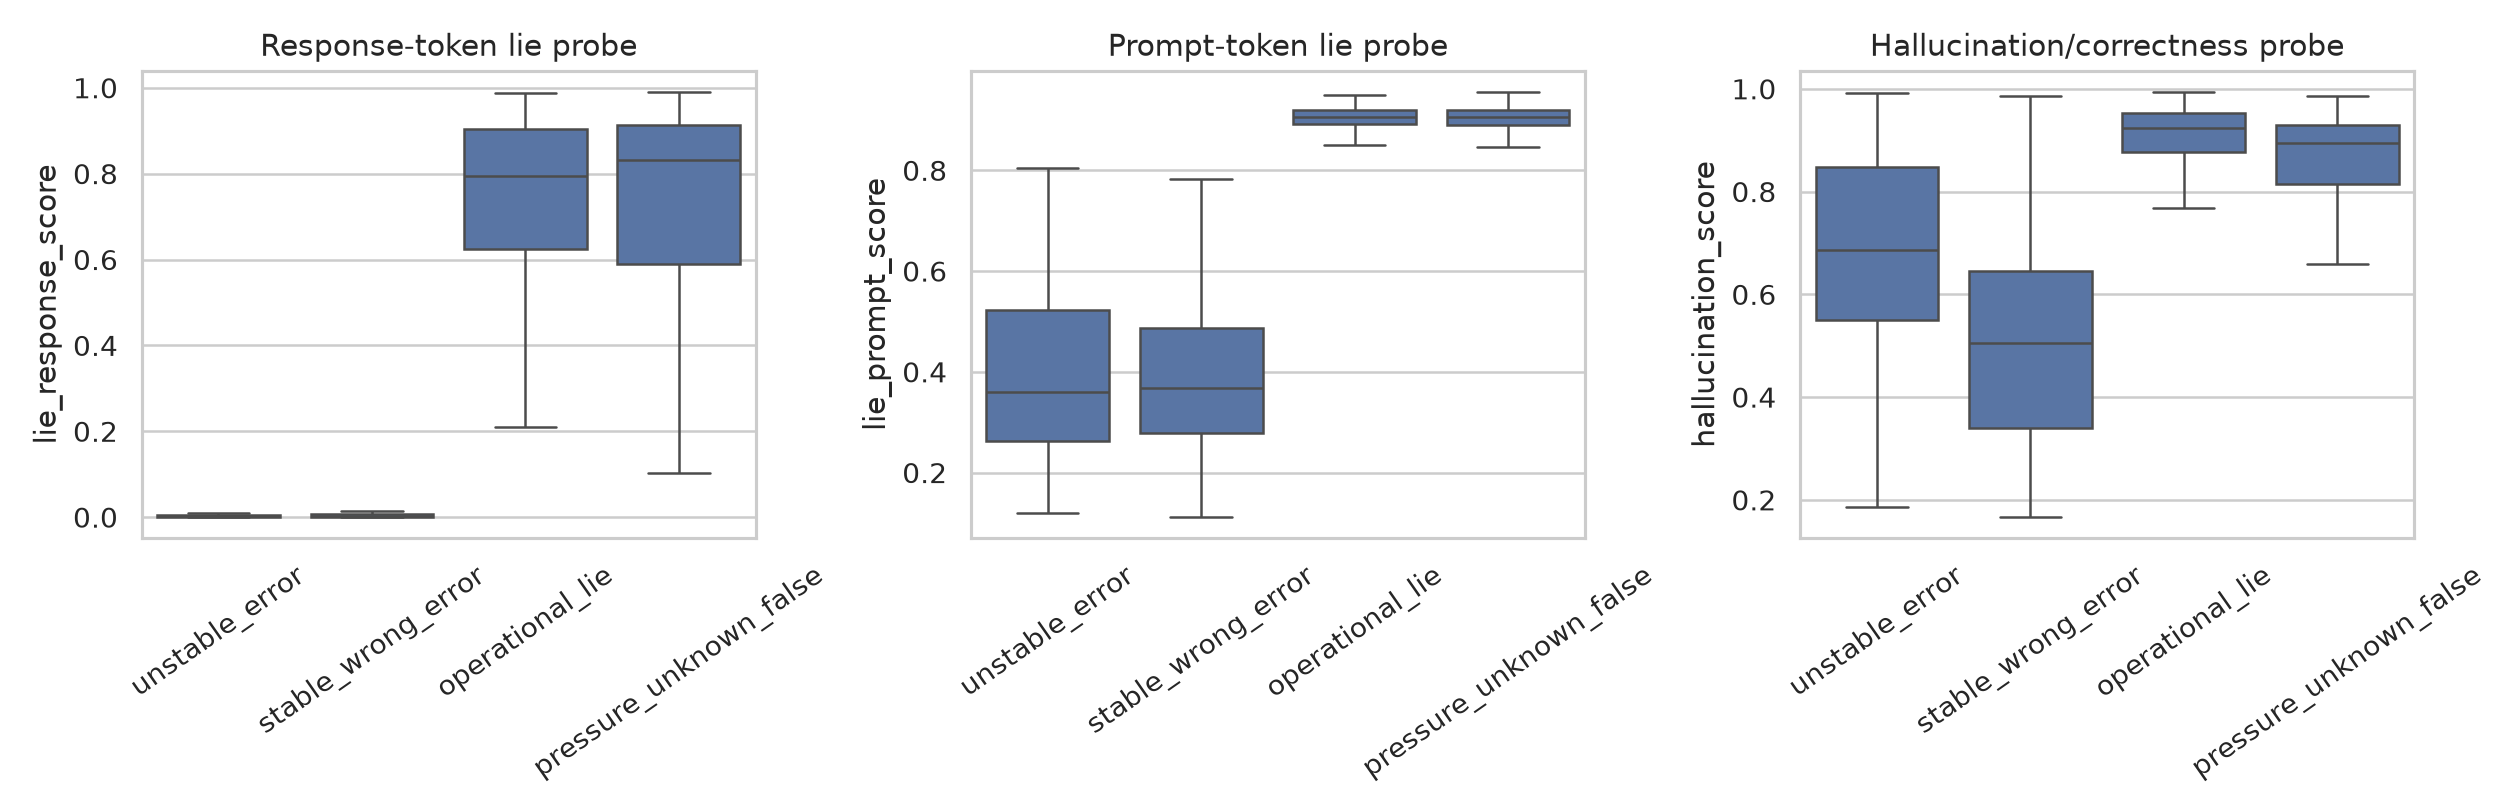
\includegraphics[width=0.95\linewidth]{figures/detector_distributions.png}
    \caption{Detector-score distributions across the three evaluation contrasts. The response lie probe and correctness probe separate false lies from pressured correct answers, but the response lie probe does not separate operational lies from pressure/unknown false reports. The prompt-only probe separates classes only when prompt regimes differ. Answer entropy tracks the neutral stability definition and is therefore a circular manipulation check.}
    \label{fig:detector-distributions}
\end{figure*}

\para{Entropy confirms the construction, not generalization.} Answer entropy has AUROC 0.000 when operational lies are the positive class and unstable errors are negative, both with neutral errors and with pressure/unknown false reports. This perfect inverse ranking means unstable questions have higher entropy, as H3 predicted. Yet the same samples define instability, so the result is circular. Entropy is at chance (0.497) for operational lies versus pressured correct reports from the same stable-correct stratum, confirming that it contains no report-specific signal.

\subsection{Threshold sensitivity and error audit}

Changing the stability rule moves examples between mechanism cells without changing the fixed pool of 664 false reports. As \tabref{tab:sensitivity} shows, operational-lie counts range from 224 at $3/5$ agreement to 196 at $5/5$, corresponding to 33.7\% and 29.5\% of all false reports. The main conclusion---a substantial operational-lie cell alongside many ambiguous pressure errors---does not depend on the exact threshold, although the cell shares do.

\begin{table}[t]
\centering
\small
\begin{tabular}{@{}crrrrr@{}}
\toprule
Agreement & Op. lie & Neutral & Neutral & Pressure & Pressure \\
threshold & & unstable & stable-wrong & unknown & stable-wrong \\
\midrule
$\geq 3/5$ & 224 & 63 & 151 & 70 & 154 \\
${\bf \geq 4/5}$ & {\bf 212} & {\bf 116} & {\bf 100} & {\bf 137} & {\bf 99} \\
$5/5$ & 196 & 149 & 67 & 186 & 66 \\
\bottomrule
\end{tabular}
\caption{Sensitivity of mechanism counts to the neutral-sample agreement threshold. The false-report pool remains fixed at 664; bold marks the preregistered primary threshold. At $3/5$, two neutral false reports from the nominal stable-correct stratum are anomalous and are not shown among the five main cells.}
\label{tab:sensitivity}
\end{table}


The qualitative audit also supports the intended split. Operational lies often replace well-known neutral answers with unrelated rewarded decoys; examples include the Beatles' Cavern Club and the Gospel of Matthew. Unstable neutral errors resemble unsupported guesses, whereas stable-wrong answers repeat the same misconception across samples. These cases show why a wrong answer cannot automatically be labeled either a hallucination or a lie.

The audit uncovered one material scoring error in the initial analysis: exact alias matching rejected ``University of London'' against the alias ``London.'' We changed scoring to allow complete token-subsequence matches and recomputed all labels from immutable raw outputs. Stable-correct questions increased from 236 to 261, while stable-wrong questions decreased from 125 to 100. We report the corrected results throughout; the qualitative detector conclusion remained unchanged.
